\documentclass[a4paper, 11pt]{article}
\usepackage{geometry}
\usepackage{graphicx}
\usepackage{a4wide}
\usepackage{ulem}
\usepackage{amsthm}
\usepackage{amsmath}
\usepackage{amsfonts}
\usepackage{amssymb}
\usepackage[T1]{fontenc}
\usepackage{ngerman}
\usepackage{graphicx}
\usepackage{epic}
\usepackage{enumerate}
\usepackage{tabu}
\usepackage [latin1]{inputenc}
\geometry{a4paper,left=15mm,right=25mm,top=20mm,bottom=25mm}
%\renewcommand{\baselinestretch}{1.5}
\newcommand{\ol}{\overline}
\newcommand{\makeline}{\hrule\vspace{5pt}}
\newcommand{\ip}[2]{\left< #1, #2 \right>}

\title{7. �bungsblatt zu Software Qualit�t}
\author{Michel Meyer, Manuel Schwarz}

\begin{document}
  \maketitle

  \section*{Aufgabe 7.1}
  \subsection*{(a)}
  %\begin{figure}
		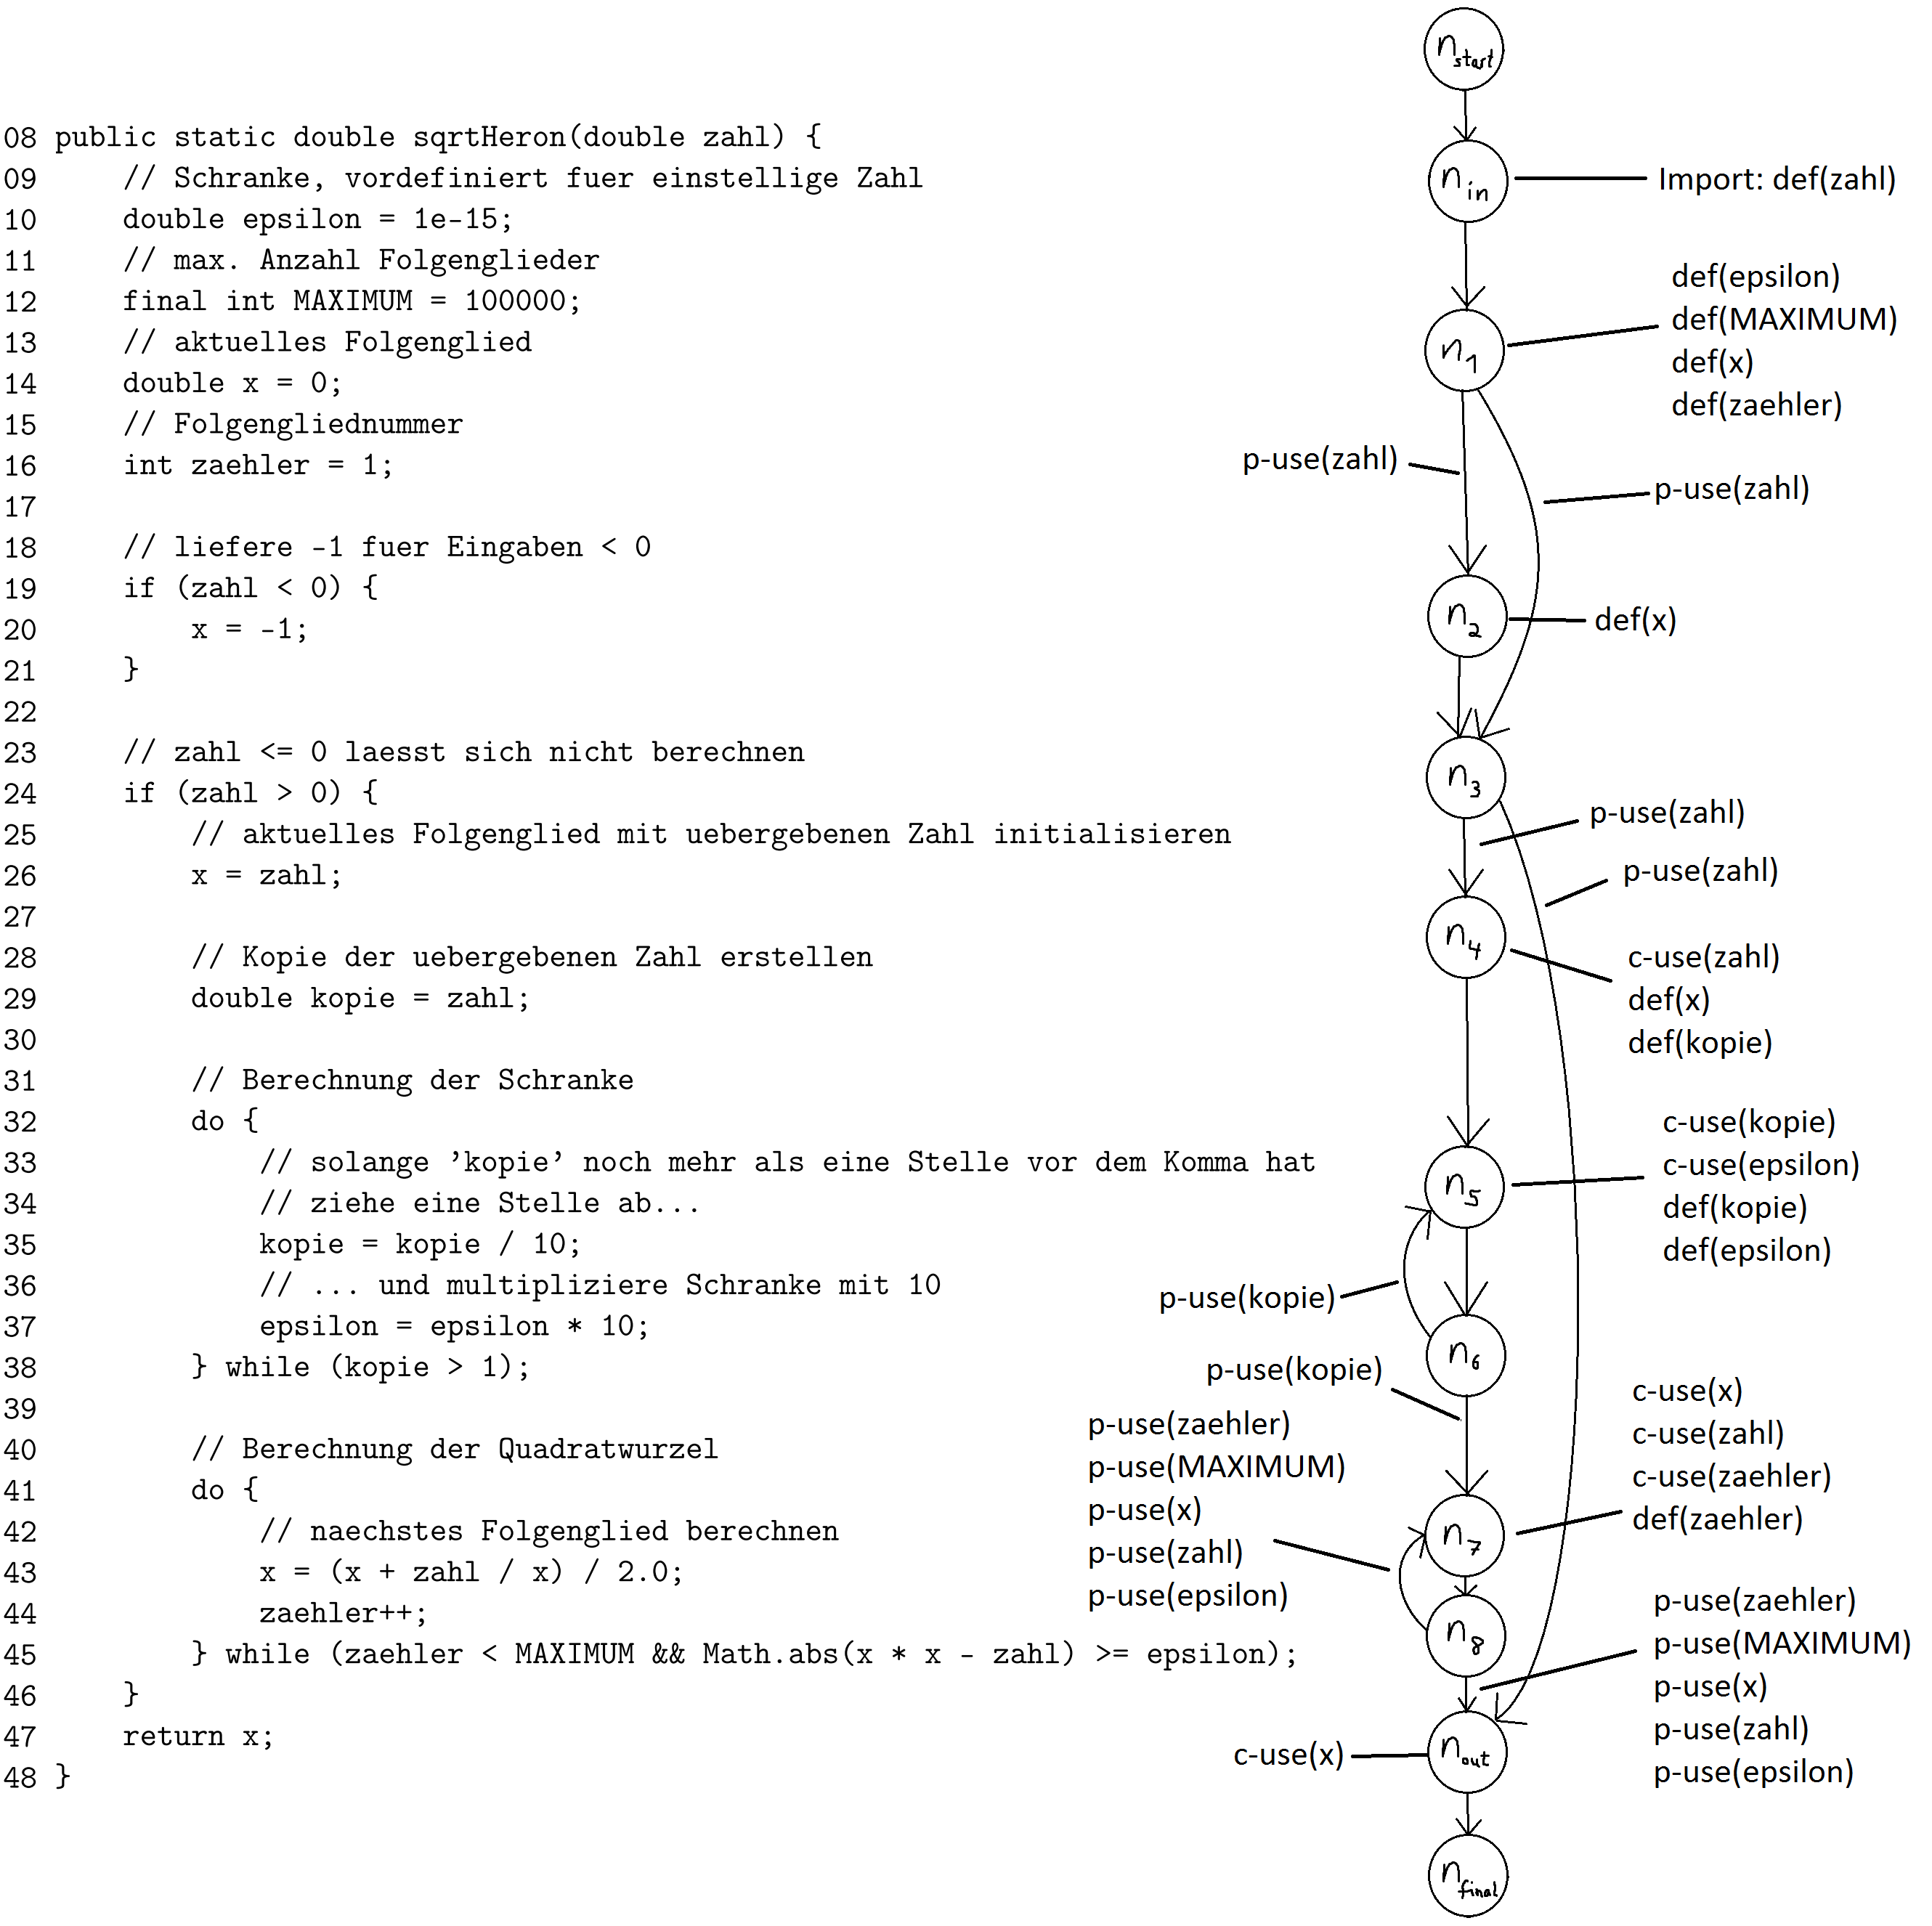
\includegraphics[width=\columnwidth]{Aufg1a.png}
	%\end{figure}
	\newpage
	\subsection*{\textit{dcu} und \textit{dpu}}
	\begin{tabular}{|l|l|l|l|}\hline
		\textbf{Variable} & \textbf{Knoten $n_i$} & \textbf{\textit{dcu($x, n_i$)}} & \textbf{\textit{dpu($x, n_i$)}} \\\hline\hline
		\texttt{zahl}    & $n_{in}$ & \{$n_4, n_7$\}        & \{$(n_1, n_2), (n_1, n_3), (n_3, n_4), (n_3, n_{out}), (n_8, n_7), (n_8, n_{out})$\} \\\hline
		\texttt{epsilon} & $n_1$    & \{$n_5$\}             & \{\} \\\hline
		\texttt{epsilon} & $n_5$    & \{$n_5$\}             & \{$(n_8, n_7), (n_8, n_{out})$\} \\\hline
		\texttt{MAXIMUM} & $n_1$    & \{\}                & \{$(n_8, n_7), (n_8, n_{out})$\} \\\hline
		\texttt{x}       & $n_1$    & \{$n_{out}$\}         & \{\} \\\hline
		\texttt{x}       & $n_2$    & \{$n_{out}$\}         & \{\} \\\hline
		\texttt{x}       & $n_4$    & \{$n_7, {n_{out}}$\}  & \{$(n_8, n_7), (n_8, n_{out})$\} \\\hline
		\texttt{zaehler} & $n_1$    & \{$n_7$\}             & \{\} \\\hline
		\texttt{zaehler} & $n_7$    & \{$n_7$\}             & \{$(n_8, n_7), (n_8, n_{out})$\} \\\hline
		\texttt{kopie}   & $n_4$    & \{$n_5$\}             & \{\} \\\hline
		\texttt{kopie}   & $n_5$    & \{$n_5$\}             & \{$(n_6, n_5), (n_6, n_7)$\} \\\hline
	\end{tabular}
	\subsection*{(b) \textit{All-defs}}
		Die Menge
		\begin{align*}
			\{(n_{start}, n_{in}, n_1, n_2, n_3, n_4, n_5, n_6, n_7, n_8, n_{out}, n_{final})\}
		\end{align*}
		testet alle definierten Variablen mindestens einmal mit \textit{c-use} oder \textit{p-use}.\\
		Der eine Pfad reicht aus, denn:
		\begin{enumerate}
			\item Mindestens ein Knoten aus jeder \textit{dcu}-Menge kommt in dem Pfad vor, womit die Definition aller Variablen au�er \texttt{MAXMIMUM} durch ein \textit{c-use} getestet wurde.
			\item F�r \texttt{MAXIMUM} ist meindestens einer der Kanten aus der \textit{dpu}-Menge im Pfad vorhanden.
		\end{enumerate}
		Allerdings gibt es keine Werte f�r die Eingabedaten, die diesen Pfad erm�glichen.
	\subsection*{(c) \textit{All-p-uses}}
		Die Menge
		\begin{align*}
			\{ & (n_{start}, n_{in}, n_1, n_2, n_3, n_4, n_5, n_6, n_7, n_8, n_{out}, n_{final}), \\
			   & (n_{start}, n_{in}, n_1, n_3, n_{out}, n_{final}), \\
			   & (n_{start}, n_{in}, n_1, n_3, n_4, n_5, n_6, n_5, n_6, n_7, n_8, n_7, n_8, n_{out}, n_{final})\}
		\end{align*}
		testet zu allen definierten Variablen alle \textit{p-uses}.\\
		Es muss gelten:
		\begin{enumerate}
			\item Zu jeder Variablen $x$ und zu jedem Knoten $n_i$ muss f�r jede Kante $(n_j, n_k) \in dpu(x, n_i)$ ein Pfad existieren, in dem diese Kante vorkommt.
			\item In dem Pfad, in dem die Kante $(n_j, n_k)$ vorkommt, muss der entsprechende Knoten $n_i$ vorher vorgekommen sein.
			\item Es muss ein definitionsfreier Pfad von $n_i$ zu $x$ bis zur Kante $(n_j, n_k)$ existieren.
		\end{enumerate}
		Eingabedaten:\\
		N/A\\
		$zahl=0$\\
		$zahl=100$
	\subsection*{(d) \textit{All-c-uses}}
		Die Menge
		\begin{align*}
			\{ & (n_{start}, n_{in}, n_1, n_2, n_3, n_4, n_5, n_6, n_5, n_6, n_7, n_8, n_7, n_8, n_{out}, n_{final}), \\
			   & (n_{start}, n_{in}, n_1, n_2, n_3, n_{out}, n_{final}), \\
			   & (n_{start}, n_{in}, n_1, n_3, n_{out}, n_{final})\}
		\end{align*}
		testet zu allen definierten Variablen alle \textit{c-uses}.\\
		Es muss gelten:
		\begin{enumerate}
			\item Zu jeder Variablen $x$ und zu jedem Knoten $n_i$ muss f�r jeden Knoten $n_j \in dcu(x, n_i)$ ein Pfad existieren, in dem dieser Knoten vorkommt.
			\item In dem Pfad, in dem der Knoten $n_j$ vorkommt, muss der entsprechende Knoten $n_i$ vorher vorgekommen sein.
			\item Es muss ein definitionsfreier Pfad von $n_i$ zu $x$ bis zum Knoten $n_j$ existieren.
		\end{enumerate}
		Eingabedaten:\\
		N/A\\
		$zahl=-1$\\
		$zahl= 0$
	\subsection*{(e) \textit{All-c-some-p-uses}}
		Die Menge aus (d) kann hier �bernommen werden, da die Menge nur um einen Pfad mit einem \textit{p-use} f�r \texttt{MAXIMUM} erweitert werden m�sste, jedoch ist die Kante $(n_8, n_{out})$ bereits im ersten Pfad vorhanden.\\
		Dass f�r \texttt{MAXIMUM} ein \textit{p-use}-Test gemacht werden muss, ist an der leeren Menge im \textit{dcu} f�r \texttt{MAXIMUM} erkennbar.
	\subsection*{(f) \textit{All-p-some-c-uses}}
		Die Menge aus (c) muss hier um einen Pfad erweitert werden.\\
		Ein \textit{c-use}-Test f�r die Definition von \texttt{epsilon} in $n_1$ ist im ersten Pfad enthalten.\\
		Ein \textit{c-use}-Test f�r die Definition von \texttt{x} in $n_1$ ist im zweiten Pfad enthalten.\\
		Ein \textit{c-use}-Test f�r die Definition von \texttt{zaehler} in $n_1$ ist im ersten Pfad enthalten.\\
		Ein \textit{c-use}-Test f�r die Definition von \texttt{kopie} in $n_4$ ist im ersten Pfad enthalten.\\
		Jedoch muss ein vierter Pfad f�r den \textit{c-use}-Test der Definition von \texttt{x} in $n_2$ hinzugef�gt werden:
			\begin{align*}
				\{ & (n_{start}, n_{in}, n_1, n_2, n_3, n_4, n_5, n_6, n_7, n_8, n_{out}, n_{final}), \\
				   & (n_{start}, n_{in}, n_1, n_3, n_{out}, n_{final}), \\
				   & (n_{start}, n_{in}, n_1, n_3, n_4, n_5, n_6, n_5, n_6, n_7, n_8, n_7, n_8, n_{out}, n_{final}), \\
				   & (n_{start}, n_{in}, n_1, n_2, n_3, n_{out}, n_{final}) \}
			\end{align*}
		F�r jede Variablendefinition, die im \textit{dpu} eine leere Menge hat, muss ein \textit{c-use}-Testfall hinzugef�gt werden. Vier von f�nf F�lle sind bereits durch den \textit{all-p-uses} abgedeckt, einer kam noch hinzu.\\
		Eingabedaten:\\
		N/A\\
		$zahl=0$\\
		$zahl=100$\\
		$zahl= -1$
	\subsection*{(g) \textit{All-uses}}
		Da das \textit{All-uses}-Kriterium eine Kombination aus den Kriterien aus (e) und (f) ist, reicht es, die Vereinigung aus beiden Mengen zu nehmen:
		\begin{align*}
				\{ & (n_{start}, n_{in}, n_1, n_2, n_3, n_4, n_5, n_6, n_7, n_8, n_{out}, n_{final}), \\
				   & (n_{start}, n_{in}, n_1, n_3, n_{out}, n_{final}), \\
				   & (n_{start}, n_{in}, n_1, n_3, n_4, n_5, n_6, n_5, n_6, n_7, n_8, n_7, n_8, n_{out}, n_{final}), \\
				   & (n_{start}, n_{in}, n_1, n_2, n_3, n_{out}, n_{final}), \\
				   & (n_{start}, n_{in}, n_1, n_2, n_3, n_4, n_5, n_6, n_5, n_6, n_7, n_8, n_7, n_8, n_{out}, n_{final})\}
		\end{align*}
		Eingabedaten:\\
		N/A\\
		$zahl=0$\\
		$zahl=100$\\
		$zahl= -1$\\
		N/A
  \subsection*{(h) \textit{All-du-uses}}
    In userem Fall ist das \textit{All-du-uses}-Kriterium deckungsgleich mit dem Fall (d).
		Die Menge
		\begin{align*}
			\{& (n_{start}, n_{in}, n_1, n_2, n_3, n_4, n_5, n_6, n_5, n_6, n_7, n_8, n_7, n_8, n_{out}, n_{final}), \\
        & (n_{start}, n_{in}, n_1, n_2, n_3, n_4, n_5, n_6, n_7, n_8, n_{out}, n_{final}), \\
        & (n_{start}, n_{in}, n_1, n_2, n_3, n_4, n_5, n_6, n_5, n_6, n_7, n_8, n_{out}, n_{final}), \\
        & (n_{start}, n_{in}, n_1, n_2, n_3, n_4, n_5, n_6, n_7, n_8, n_7, n_8, n_{out}, n_{final}), \\
			  & (n_{start}, n_{in}, n_1, n_3, n_4, n_5, n_6, n_5, n_6, n_7, n_8, n_7, n_8, n_{out}, n_{final}), \\
        & (n_{start}, n_{in}, n_1, n_3, n_4, n_5, n_6, n_7, n_8, n_{out}, n_{final}), \\
        & (n_{start}, n_{in}, n_1, n_3, n_4, n_5, n_6, n_5, n_6, n_7, n_8, n_{out}, n_{final}), \\
        & (n_{start}, n_{in}, n_1, n_3, n_4, n_5, n_6, n_7, n_8, n_7, n_8, n_{out}, n_{final}), \\
			  & (n_{start}, n_{in}, n_1, n_2, n_3, n_{out}, n_{final}), \\
			  & (n_{start}, n_{in}, n_1, n_3, n_{out}, n_{final})\}
		\end{align*}
		Eingabedaten:\\
		N/A\\
		N/A\\
		N/A\\
		N/A\\
		$zahl=100$\\
		$zahl=1$\\
		N/A\\
		N/A\\
		$zahl= -1$\\
		$zahl=0$\\
		testet alle \textit{du}-Pfade bez�glich aller Definitionen aller Variablen.\\
\end{document}
